\section{Use Case Diagram}
\begin{figure}[h]
	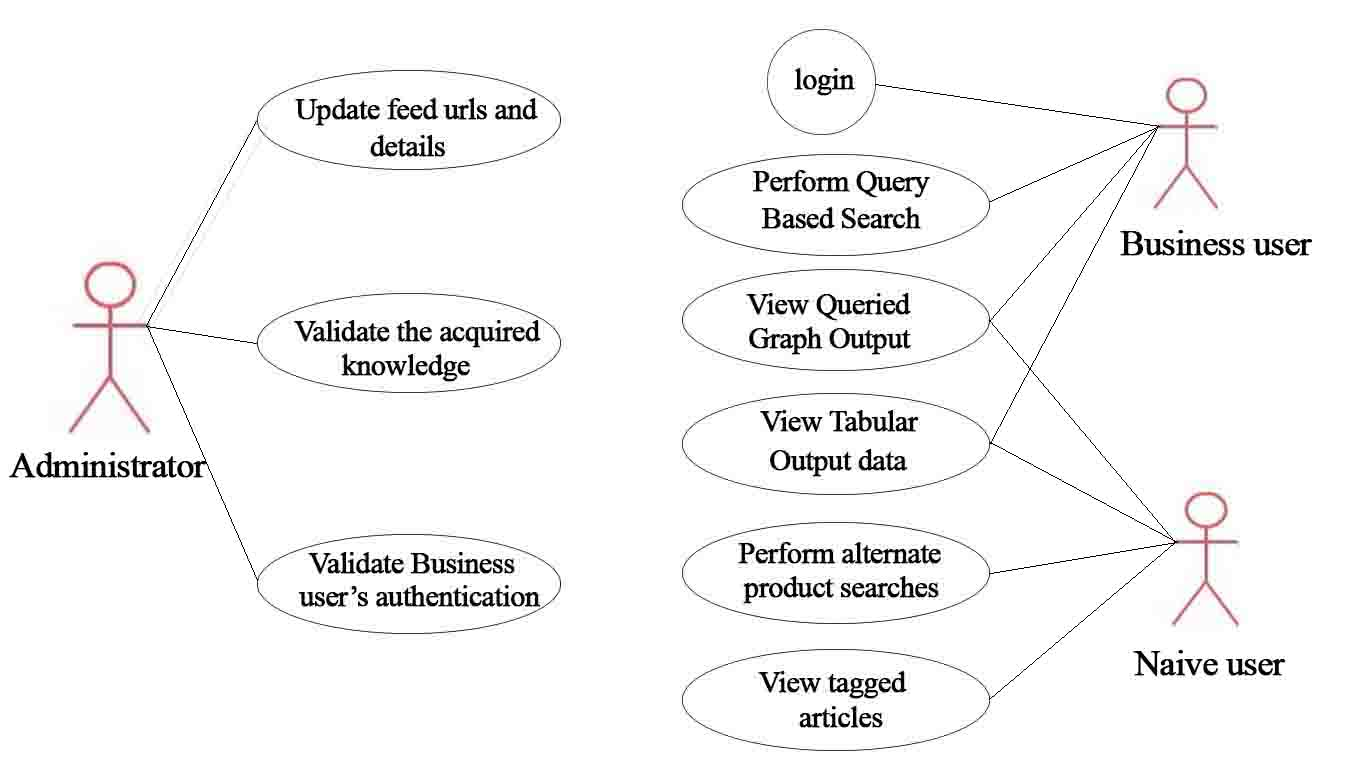
\includegraphics[width=13cm, height=7cm]{usecase}
	\centering
	\caption{Use case Diagram}
\end{figure}
\newpage
\section{Data Flow Diagram}
\begin{figure}[h]
	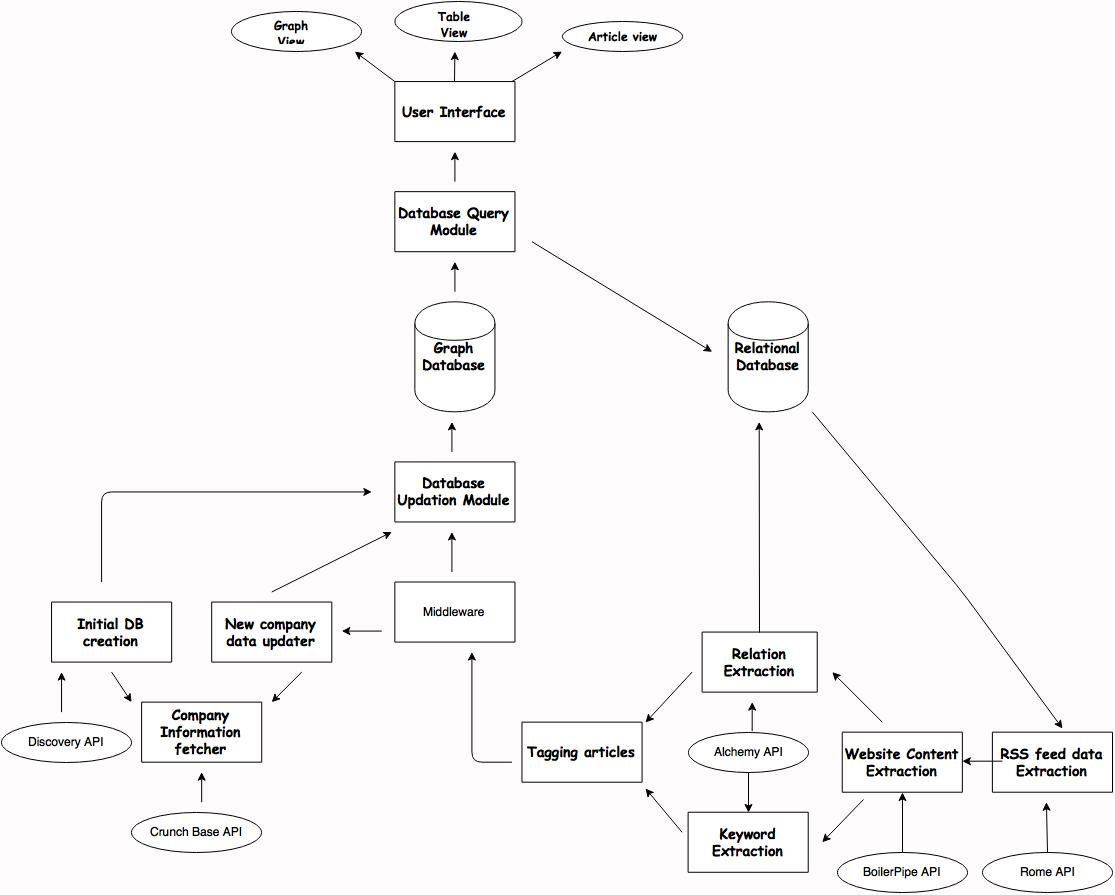
\includegraphics[width=10cm, height=11cm]{dataflow}
	\centering
	\caption{Data Flow Diagram Diagram}
\end{figure}
\newpage
\section{Database design}
\par There are two types of database systems used they are 
\begin{itemize}
\item Graph database 
\item Object-Relational database
\end{itemize}

\subsection{Graph database}
\par 
In computing, a graph database is a database that uses graph structures for semantic queries with nodes, edges and properties to represent and store data. A key concept of the system is the graph (or edge or relationship), which directly relates data items in the store. This contrasts with conventional relational databases, where links between data are ad hoc and based on the data itself, and related items are gathered by searching for this data within the store. Graph databases are designed to allow simple and rapid retrieval of complex hierarchical structures, whereas a relational database would use a complex query to achieve the same end, generally with far less performance.
\par The underlying storage mechanism of graph database products varies. Some, like Maria DB, are based on a relational engine and store the graph data in a table. More common examples generally use a key-value store or document-oriented database for storage, making them inherently NoSQL solutions. These solutions generally offer a performance advantage because the graph is stored in a format similar to a database index, minimizing its size and retrieval time. Most graph databases based on non-relational storage engines also add the concept of tags or properties, which are essentially relationships lacking a pointer to another document. This allows data elements to be categorized for easy retrieval in mass. Examples of NoSQL graph databases include Orient DB, Neo4j and Arango DB.
\par The Graph database in use is Neo4j. It is a graph database management system developed by Neo Technology, Inc. Described by its developers as an ACID-compliant transactional database with native graph storage and processing, Neo4j is the most popular graph database according to db-engines.com.
\par Neo4j is available in a GPL3-licensed open-source "community edition", with online backup and high availability extensions licensed under the terms of the Affero General Public License. Neo also licenses Neo4j with these extensions under closed-source commercial terms.
\par Neo4j is implemented in Java and accessible from software written in other languages using the Cypher Query Language through a transactional HTTP endpoint.
 \par The graph database schema in use is depicted in the Figure \ref{fig:graphdatabaseschema}

\begin{figure}[h]
	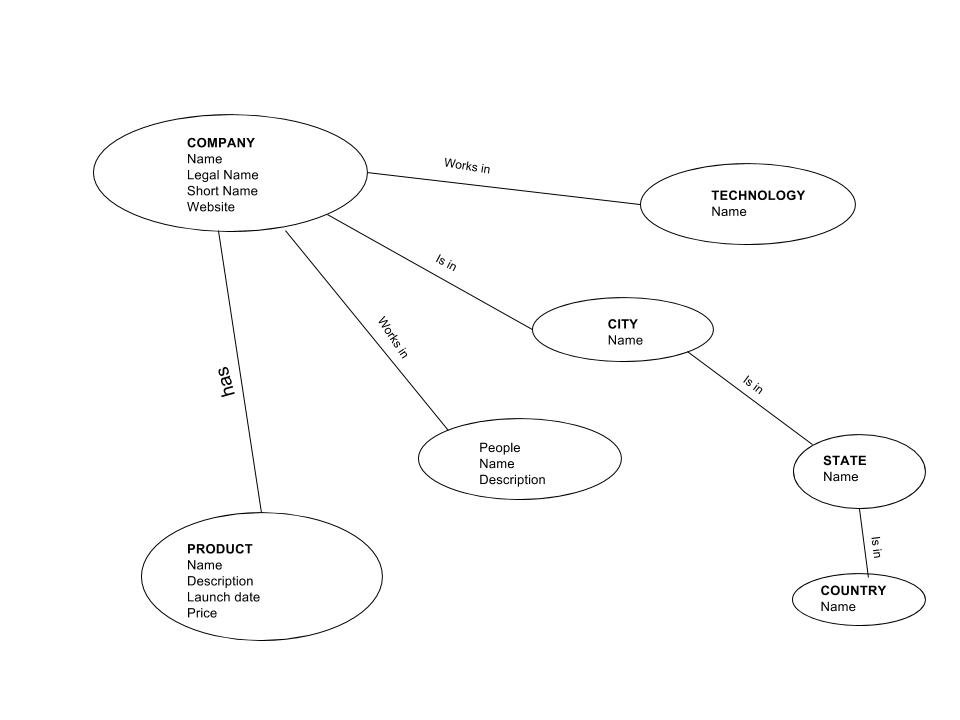
\includegraphics[width=10cm, height=11cm]{graphdatabaseschema}
	\centering
	\caption{The graph database schema}
	\label{fig:graphdatabaseschema}
\end{figure}

\subsection{Object-Relational database system}

\par An object-relational database (ORD), or object-relational database management system (ORDBMS), is a database management system (DBMS) similar to a relational database, but with an object-oriented database model: objects, classes and inheritance are directly supported in database schemas and in the query language. In addition, just as with pure relational systems, it supports extension of the data model with custom data-types and methods.
\par An object-relational database can be said to provide a middle ground between relational databases and object-oriented databases (object database). In object-relational databases, the approach is essentially that of relational databases: the data resides in the database and is manipulated collectively with queries in a query language; at the other extreme are OODBMS’s in which the database is essentially a persistent object store for software written in an object-oriented programming language, with a programming API for storing and retrieving objects, and little or no specific support for querying.
\par The ORDBMS in use is PostgreSQL, often simply PostgreSQL, is an object-relational database management system (ORDBMS) with an emphasis on extensibility and standards-compliance. As a database server, its primary function is to store data securely, supporting best practices, and to allow for retrieval at the request of other software applications. It can handle workloads ranging from small single-machine applications to large Internet-facing applications with many concurrent users.
\\
\par PostgreSQL implements the majority of the core SQL: 2011 standard, is ACID-compliant and transactional (including most DDL statements) avoiding locking issues using multi version concurrency control (MVCC), provides immunity to dirty reads and full serializability. handles complex SQL queries using many indexing methods that are not available in other databases; has updateable views and materialized views, triggers, foreign keys; supports functions and stored procedures, and other expandability, and has a large number of extensions written by third parties. In addition to the possibility of working with the major proprietary and open source databases, PostgreSQL supports migration from them, by its extensive standard SQL support and available migration tools. Proprietary extensions in databases such as Oracle can be emulated by built-in and third-party open source compatibility extensions. Recent versions also provide replication of the database itself for availability and scalability.
\par
PostgreSQL is cross-platform and runs on many operating systems including Linux, FreeBSD, OS X, Solaris, and Microsoft Windows. On OS X, PostgreSQL has been the default database starting with Mac OS X 10.7 Lion Server, and PostgreSQL client tools are bundled within the desktop edition. The vast majority of Linux distributions have it available in supplied packages.
\par PostgreSQL is developed by the PostgreSQL Global Development Group, a diverse group of many companies and individual contributors. It is free and open-source software, released under the terms of the PostgreSQL License, a permissive free-software license.
\par The schemas of the relations used in PostgreSQL are
\begin{itemize}
\item Feed (feed\_id, url, last\_accessed\_time)
\item Article (url, heading, taxonomy, context)
\item Temporary\_Relation (id, statement, subject\_text, subject\_text, object\_text, object\_type, verb\_text, context) 
\item Relations (relation\_id, statement, subject\_text, subject\_text, object\_text, object\_type, verb\_text, context) 
\item Taxonomy\_word (word, taxonomy)
\item Context\_work (word, context)
\item Taxonomy\_code (code, taxonomy)
\item Context\_code (code, context)
\item Company (website, name, legal\_name, short\_name)
\item Technology (name)
\item Works\_in (website, name)
\item City (name)
\item State (name)
\item Country (name)
\item Is\_at (website, name)
\item Is\_in (name, name)
\item Product (product\_id, name, launch\_date, description, price)
\item Has (website, product\_id)
\item Person (person\_id, first\_name, second\_name, designation)
\item Works\_in (person\_id, website)
\end{itemize}

\section{User interface design}
\par 
User interface is the front-end application view to which user interacts in order to use the software. User can manipulate and control the software as well as hardware by means of user interface. Today, user interface is found at almost every place where digital technology exists, right from computers, mobile phones, cars, music players, airplanes, ships etc.
\par User interface is part of software and is designed such a way that it is expected to provide the user insight of the software. UI provides fundamental platform for human-computer interaction.
\par UI can be graphical, text-based, audio-video based, depending upon the underlying hardware and software combination. UI can be hardware or software or a combination of both.

The software becomes more popular if its user interface is:
\begin{itemize}
\item Attractive
\item Simple to use
\item Responsive in short time
\item Clear to understand
\item Consistent on all interfacing screens
\end{itemize}
UI is broadly divided into two categories:
\begin{itemize}
\item Command Line Interface
\item Graphical User Interface
\end{itemize}
\subsection{Different user interfaces}
\par There are three separate user interfaces implemented for the use of different kinds of users they are 
\begin{itemize}
\item Naïve user
\item Business user
\item Administrator
\end{itemize}
\subsubsection{For the naive user}
\par The list of all articles that has been fetched by Dynamic data collector is listed here for the naïve user’s reference this is categorized according to their tags.  A synopsis of the article is provided in here itself, the interested user can follow the link to the original article.
\subsubsection{For the business user}
\par The business user can query the graph database to get a variety of predefined relations. The results may be shown either as the graph visualization or as a tabular representation according to the type of query.
\subsubsection{For the administrator}
\par The administrator interface lists the relations that are extracted by the Dynamic data extractor. Each relations will have subject, subject type, object, object type predicate, and predicate type. The sentence from which these relations are extracted are shown for verification. This will allow the filtering of duplicate as well as junk data.